One could also define quadratic Bezier curves. These have only a
single control point, and the curve is such that in both the endpoints
it is aimed at the control point.\\
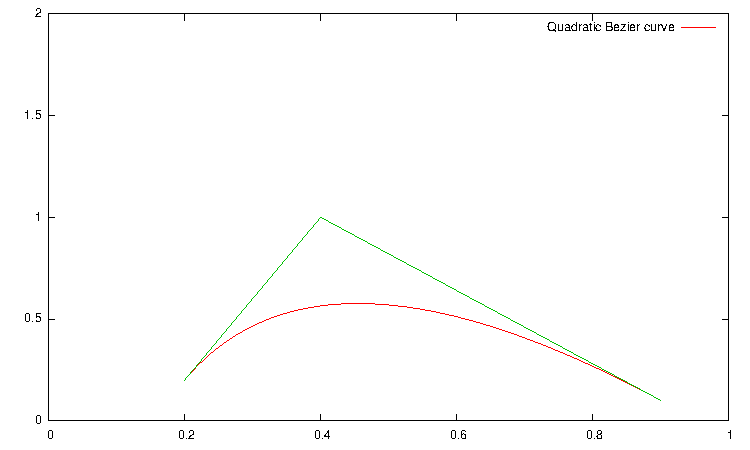
\includegraphics{bquad}\\
Derive the basis functions and geometry matrix for this case.
Make a \gnuplot\ figure of a single quadratic Bezier curve, and of two
curves joined smoothly.

Hint: you can follow the construction of the cubic splines in the
lecture notes. The only
problem is defining the control point. First draw up the Hermite geometry matrix
based on end points $q_0$ and~$q_1$, and the derivative $q_0'$ in the
first end point. Derive from them the derivative~$q_1'$ in the other
end point. The control point then lies on the intersection of two
lines. Solving this looks like a single equation in two unknowns, but
it can be solved: write it as a matrix-vector equation that is
satisfied no matter the choice of the geometry matrix.
